\documentclass[10pt]{article}
\usepackage[T1]{fontenc}

% Document Details
\newcommand{\CLASS}{AMATH 584}
\newcommand{\assigmentnum}{Assignment 7}

\usepackage[margin = 1.15in, top = 1.25in, bottom = 1.in]{geometry}

\usepackage{titling}
\setlength{\droptitle}{-6em}   % This is your set screw
\date{}
\renewcommand{\maketitle}{
	\clearpage
	\begingroup  
	\centering
	\LARGE \sffamily\textbf{\CLASS} \Large \assigmentnum\\[.8em]
	\large Tyler Chen\\[1em]
	\endgroup
	\thispagestyle{empty}
}
 % Title Styling
\usepackage{tocloft}
\renewcommand{\cfttoctitlefont}{\Large\sffamily\bfseries}
\renewcommand{\cftsecfont}{\normalfont\sffamily\bfseries}
\renewcommand{\cftsubsecfont}{\normalfont\sffamily}
\renewcommand{\cftsubsubsecfont}{\normalfont\sffamily}

\makeatletter
\let\oldl@section\l@section
\def\l@section#1#2{\oldl@section{#1}{\sffamily\bfseries#2}}

\let\oldl@subsection\l@subsection
\def\l@subsection#1#2{\oldl@subsection{#1}{\sffamily#2}}

\let\oldl@subsubsection\l@subsubsection
\def\l@subsubsection#1#2{\oldl@subsubsection{#1}{\sffamily#2}}
 % General Styling


\usepackage{enumitem}

% Figures
\usepackage{subcaption}

% TikZ and Graphics
\usepackage{tikz, pgfplots}
\pgfplotsset{compat=1.12}
\usetikzlibrary{patterns,arrows}
\usepgfplotslibrary{fillbetween}

\usepackage{pdfpages}
\usepackage{adjustbox}

\usepackage{lscape}
\usepackage{titling}
\usepackage[]{hyperref}


% Header Styling
\usepackage{fancyhdr}
\pagestyle{fancy}
\lhead{\sffamily \CLASS}
\rhead{\sffamily Chen \textbf{\thepage}}
\cfoot{}

% Paragraph Styling
\setlength{\columnsep}{1cm}
\setlength{\parindent}{0pt}
\setlength{\parskip}{5pt}
\renewcommand{\baselinestretch}{1}

% TOC Styling
\usepackage{tocloft}
\iffalse
\renewcommand{\cftsecleader}{\cftdotfill{\cftdotsep}}

\renewcommand\cftchapafterpnum{\vskip6pt}
\renewcommand\cftsecafterpnum{\vskip10pt}
\renewcommand\cftsubsecafterpnum{\vskip6pt}

% Adjust sectional unit title fonts in ToC
\renewcommand{\cftchapfont}{\sffamily}
\renewcommand{\cftsecfont}{\bfseries\sffamily}
\renewcommand{\cftsecnumwidth}{2em}
\renewcommand{\cftsubsecfont}{\sffamily}
\renewcommand{\cfttoctitlefont}{\hfill\bfseries\sffamily\MakeUppercase}
\renewcommand{\cftaftertoctitle}{\hfill}

\renewcommand{\cftchappagefont}{\sffamily}
\renewcommand{\cftsecpagefont}{\bfseries\sffamily}
\renewcommand{\cftsubsecpagefont}{\sffamily}
\fi
 % General Styling
% Code Display Setup
\usepackage{listings,lstautogobble}
\usepackage{lipsum}
\usepackage{courier}
\usepackage{catchfilebetweentags}

\lstset{
	basicstyle=\small\ttfamily,
	breaklines=true, 
	frame = single,
	rangeprefix=,
	rangesuffix=,
	includerangemarker=false,
	autogobble = true
}


\usepackage{algorithmicx}
\usepackage{algpseudocode}

\newcommand{\To}{\textbf{to}~}
\newcommand{\DownTo}{\textbf{downto}~}
\renewcommand{\algorithmicdo}{\hspace{-.2em}\textbf{:}}
 % Code Display Setup
% AMS MATH Styling
\usepackage{amsmath, amssymb}
\newcommand{\qed}{\hfill\(\square\)}

%\newtheorem*{lemma}{Lemma} 
%\newtheorem*{theorem}{Theorem}
%\newtheorem*{definition}{Definition}
%\newtheorem*{prop}{Proposition}
%\renewenvironment{proof}{{\bfseries Proof.}}{}


% mathcal
\newcommand{\cA}{\ensuremath{\mathcal{A}}}
\newcommand{\cB}{\ensuremath{\mathcal{B}}}
\newcommand{\cC}{\ensuremath{\mathcal{C}}}
\newcommand{\cD}{\ensuremath{\mathcal{D}}}
\newcommand{\cE}{\ensuremath{\mathcal{E}}}
\newcommand{\cF}{\ensuremath{\mathcal{F}}}
\newcommand{\cG}{\ensuremath{\mathcal{G}}}
\newcommand{\cH}{\ensuremath{\mathcal{H}}}
\newcommand{\cI}{\ensuremath{\mathcal{I}}}
\newcommand{\cJ}{\ensuremath{\mathcal{J}}}
\newcommand{\cK}{\ensuremath{\mathcal{K}}}
\newcommand{\cL}{\ensuremath{\mathcal{L}}}
\newcommand{\cM}{\ensuremath{\mathcal{M}}}
\newcommand{\cN}{\ensuremath{\mathcal{N}}}
\newcommand{\cO}{\ensuremath{\mathcal{O}}}
\newcommand{\cP}{\ensuremath{\mathcal{P}}}
\newcommand{\cQ}{\ensuremath{\mathcal{Q}}}
\newcommand{\cR}{\ensuremath{\mathcal{R}}}
\newcommand{\cS}{\ensuremath{\mathcal{S}}}
\newcommand{\cT}{\ensuremath{\mathcal{T}}}
\newcommand{\cU}{\ensuremath{\mathcal{U}}}
\newcommand{\cV}{\ensuremath{\mathcal{V}}}
\newcommand{\cW}{\ensuremath{\mathcal{W}}}
\newcommand{\cX}{\ensuremath{\mathcal{X}}}
\newcommand{\cY}{\ensuremath{\mathcal{Y}}}
\newcommand{\cZ}{\ensuremath{\mathcal{Z}}}

% mathbb
\usepackage{bbm}
\newcommand{\bOne}{\ensuremath{\mathbbm{1}}}

\newcommand{\bA}{\ensuremath{\mathbb{A}}}
\newcommand{\bB}{\ensuremath{\mathbb{B}}}
\newcommand{\bC}{\ensuremath{\mathbb{C}}}
\newcommand{\bD}{\ensuremath{\mathbb{D}}}
\newcommand{\bE}{\ensuremath{\mathbb{E}}}
\newcommand{\bF}{\ensuremath{\mathbb{F}}}
\newcommand{\bG}{\ensuremath{\mathbb{G}}}
\newcommand{\bH}{\ensuremath{\mathbb{H}}}
\newcommand{\bI}{\ensuremath{\mathbb{I}}}
\newcommand{\bJ}{\ensuremath{\mathbb{J}}}
\newcommand{\bK}{\ensuremath{\mathbb{K}}}
\newcommand{\bL}{\ensuremath{\mathbb{L}}}
\newcommand{\bM}{\ensuremath{\mathbb{M}}}
\newcommand{\bN}{\ensuremath{\mathbb{N}}}
\newcommand{\bO}{\ensuremath{\mathbb{O}}}
\newcommand{\bP}{\ensuremath{\mathbb{P}}}
\newcommand{\bQ}{\ensuremath{\mathbb{Q}}}
\newcommand{\bR}{\ensuremath{\mathbb{R}}}
\newcommand{\bS}{\ensuremath{\mathbb{S}}}
\newcommand{\bT}{\ensuremath{\mathbb{T}}}
\newcommand{\bU}{\ensuremath{\mathbb{U}}}
\newcommand{\bV}{\ensuremath{\mathbb{V}}}
\newcommand{\bW}{\ensuremath{\mathbb{W}}}
\newcommand{\bX}{\ensuremath{\mathbb{X}}}
\newcommand{\bY}{\ensuremath{\mathbb{Y}}}
\newcommand{\bZ}{\ensuremath{\mathbb{Z}}}

% alternative mathbb
\newcommand{\NN}{\ensuremath{\mathbb{N}}}
\newcommand{\RR}{\ensuremath{\mathbb{R}}}
\newcommand{\CC}{\ensuremath{\mathbb{C}}}
\newcommand{\ZZ}{\ensuremath{\mathbb{Z}}}
\newcommand{\EE}{\ensuremath{\mathbb{E}}}
\newcommand{\PP}{\ensuremath{\mathbb{P}}}
\newcommand{\VV}{\ensuremath{\mathbb{V}}}
\newcommand{\cov}{\ensuremath{\text{Co}\VV}}
% Math Commands

\newcommand{\st}{~\big|~}
\newcommand{\stt}{\text{ st. }}
\newcommand{\ift}{\text{ if }}
\newcommand{\thent}{\text{ then }}
\newcommand{\owt}{\text{ otherwise }}

\newcommand{\norm}[1]{\left\lVert#1\right\rVert}
\newcommand{\snorm}[1]{\lVert#1\rVert}
\newcommand{\ip}[1]{\ensuremath{\left\langle #1 \right\rangle}}
\newcommand{\pp}[3][]{\frac{\partial^{#1}#2}{\partial #3^{#1}}}
\newcommand{\dd}[3][]{\frac{\d^{#1}#2}{\d #3^{#1}}}
\renewcommand{\d}{\ensuremath{\mathrm{d}}}

\newcommand{\indep}{\rotatebox[origin=c]{90}{$\models$}}




 % Math shortcuts
% Problem
\usepackage{floatrow}

\newenvironment{problem}[1][]
{\pagebreak
\noindent\rule{\textwidth}{1pt}\vspace{0.25em}
{\sffamily \textbf{#1}}
\par
}
{\par\vspace{-0.5em}\noindent\rule{\textwidth}{1pt}}

\newenvironment{solution}[1][]
{{\sffamily \textbf{#1}}
\par
}
{}

 % Problem Environment

\newcommand{\note}[1]{\textcolor{red}{\textbf{Note:} #1}}

\hypersetup{
   colorlinks=true,       % false: boxed links; true: colored links
   linkcolor=violet,          % color of internal links (change box color with linkbordercolor)
   citecolor=green,        % color of links to bibliography
   filecolor=magenta,      % color of file links
   urlcolor=cyan           % color of external links
}


\begin{document}
\maketitle

\begin{problem}[Exercise 1]

Write a routine to generate an \(m\) by \(m\) matrix with a given 2-norm condition
number.  You can make your routine a \verb+function+ in Matlab that takes
two input arguments -- the matrix size \(m\) and the desired condition number
\verb+condno+ -- and produces an \(m\) by \(m\) matrix \(A\) with the given condition
number as output:

\begin{verbatim}
function A = matgen(m, condno)
\end{verbatim}

Form \(A\) by generating two random orthogonal matrices \(U\) and \(V\) and a 
diagonal matrix \(\Sigma\) with \(\sigma_{jj} = \mbox{condno}^{-(j-1)/(m-1)}\),
and setting \(A = U \Sigma V^{*}\).  [Note that the largest diagonal entry
of \(\Sigma\) is \(1\) and the smallest is \(\mbox{condno}^{-1}\), so the ratio is
\verb+condno+.]  You can generate a random orthogonal matrix in Matlab by
first generating a random matrix, \verb+Mat = randn(m)+, and then computing
its QR decomposition, \verb+[Q,R] = qr(Mat)+.  The matrix \verb+Q+ is then
a random orthogonal matrix.  You can check the condition number of the
matrix you generate by using the function \verb+cond+ in Matlab.  Turn in
a listing of your code.

For \verb+condno+$= (1,~10^4 ,~10^8 , 10^{12} , 10^{16})$, use your routine
to generate a random matrix \verb+A+ with condition number \verb+condno+.
Also generate a random vector \verb+xtrue+ of length \(m\) and compute
the product \verb+b = A*xtrue+.

\begin{enumerate}
    \item[(a)]
Solve \(Ax=b\) using Gaussian elimination with partial pivoting.  This
can be done in Matlab by typing \verb+x = A\b+.  Determine the 2-norm
of the error {\tt norm(x - xtrue)/norm(xtrue)} in your computed solution and explain how this is related to the condition number of \(A\).  Compute the 2-norm of the residual, \verb+norm(b-A*x)/(norm(A)*norm(x))+.  Does the algorithm for solving \(Ax=b\) appear to be backward stable (at least for this problem); that is, is the computed solution the exact solution to a nearby problem?

\item[(b)] Solve \(Ax=b\) by inverting \(A\) and multiplying by the inverse: {\tt Ainv = inv(A); x = Ainv*b}.  Again look at relative errors and 
residuals.  Does this algorithm appear to be backward stable?

\item[(c)] Finally, solve \(Ax=b\) using Cramer's rule (i.e., compute the determinant of \(A\) by typing \verb+det(A)+ and then compute \verb+x(j)+ by replacing column \(j\) of \(A\) by the right-hand side vector \(b\), computing the determinant of the resulting matrix \(A_j\) and finding the ratio:  \verb+det(A_j)/det(A)+). Again look at relative errors and residuals and determine whether this  algorithm is backward stable.
\end{enumerate}

Turn in a table showing the relative errors and residuals for each of the three algorithms and each of the condition numbers tested, along with a  brief explanation of the results.
\end{problem}

\begin{solution}[Solution]
We implement the function \verb|matgen| in python as,
\begin{lstlisting}
def matgen(m,condno):
    [U,X] = np.linalg.qr(np.random.randn(m,m))
    [V,X] = np.linalg.qr(np.random.randn(m,m))
    S = np.diag(condno**((1-np.linspace(1,m,m))/(m-1)))
    return U@S@V
\end{lstlisting}

We implement the methods of solving as:
\begin{lstlisting}
def exercise_1():
    ge_err,inv_err,cr_err = [],[],[]
    m = 20
    for condno in [0,4,8,12,16]:
        
        A = matgen(m,10**condno)
        xtrue = np.random.rand(m)
        b = A@xtrue

        x_ge = np.linalg.solve(A,b)
        ge_err.append([condno, np.linalg.norm(x_ge-xtrue)/np.linalg.norm(xtrue),
               np.linalg.norm(b-A@x_ge)/(np.linalg.norm(A)*np.linalg.norm(x_ge))])
        
        Ainv =  np.linalg.inv(A)
        x_inv = Ainv@b
        inv_err.append([condno, np.linalg.norm(x_inv-xtrue)/np.linalg.norm(xtrue),
               np.linalg.norm(b-A@x_inv)/(np.linalg.norm(A)*np.linalg.norm(x_inv))])
    
        detA = np.linalg.det(A)
        x_cr = np.zeros(m)
        for j in range(m):
            A_j = copy.deepcopy(A)
            A_j[:,j] = b
            x_cr[j] = np.linalg.det(A_j)/detA
        cr_err.append([condno, np.linalg.norm(x_cr-xtrue)/np.linalg.norm(xtrue),
               np.linalg.norm(b-A@x_cr)/(np.linalg.norm(A)*np.linalg.norm(x_cr))])

    return [ge_err,inv_err,cr_err]
\end{lstlisting}

Note that the outputs are the condition number, the normalized error, and the normalized residual.

\begin{enumerate}
    \item[(a)] Note that the linear solver in numpy is implemented using LAPACK routine \_gesv (Gaussian elimination with partial pivoting).

        The algorithm appears backward stable since the residuals are all order \( \epsilon_{\text{mach}} \).
        \begin{lstlisting}
 [[0,   4.9733030843277515e-16, 1.0709777379963362e-16],
  [4,   1.3628659511587549e-13, 1.1343275878528474e-16],
  [8,   6.9160795579062393e-10, 2.0119792028960311e-17],
  [12,  2.999596419709301e-06,  1.7083267125104297e-17],
  [16,  0.017776866915952674,   6.8866641918714602e-17]],
        \end{lstlisting}

    \item[(b)] The algorithm appears not backward stable since the residual gets large as the condition number increases.

    \begin{lstlisting}
 [[0,   5.6668973422827896e-16, 1.1959722892476256e-16],
  [4,   3.3270648768047658e-13, 2.9990752835841747e-14],
  [8,   5.5312036797396992e-10, 1.8815131322505332e-11],
  [12,  7.8752782311348258e-06, 2.1784856442503186e-07],
  [16,  2.3924681879507204,     0.0013630213010579159]],
    \end{lstlisting}


    \item[(c)] Note that for too large of \( m \) the determinant is not properly calculated.

 The algorithm appears not backward stable since the residual gets large as the condition number increases.
        
        \begin{lstlisting}
 [[0,   7.4032045694590438e-16, 1.7619297304857857e-16],
  [4,   1.0791108088755479e-13, 1.344502372418256e-14],
  [8,   5.7468386383603836e-10, 1.0701321230827662e-10],
  [12,  4.6049547088035518e-06, 1.0994510094470615e-06],
  [16,  0.029069352525193739,   0.0041372463048906759]]
        \end{lstlisting}
\end{enumerate}
\end{solution}


\begin{problem}[Exercise 2]
In Matlab, form a \(60\) by \(60\) matrix \(A\) with \(1\)'s on the main diagonal and in the last column, with \(-1\)'s below the main diagonal, and with
\(0\)'s everywhere else, as in (22.4) on p.~165 in the text.  Compute the 2-norm condition number of \(A\):  \verb+cond(A)+.  Set a random
vector \(x\) of length \(60\):  \verb+x = randn(60,1)+.  Compute \verb+b = A*x+. 
\begin{enumerate}
    \item[(a)] Solve the linear system \(A x = b\) using Gaussian elimination with partial pivoting by typing \verb+x_ge = A\b+.  Compute the 2-norm of the difference between the computed vector \verb+x_ge+ and the true solution \verb+x+ generated previously.
    \item[(b)] Solve the linear system \(Ax=b\) using the QR factorization of \(A\): \verb+[Q,R] = qr(A);+ \verb+x_qr = R\(Q'*b)+.  Compute the 2-norm of the difference between the computed vector \verb+x_qr+ and the true solution \verb+x+.  Explain the difference in accuracy between the two computed solutions \verb+x_ge+ and \verb+x_qr+.  
    \item[(c)] By hand, factor the \(5\) by \(5\) matrix in (22.4) on p.~165 using {\em complete} pivoting, so that \(PAQ = LU\).  What is the growth factor \(\rho\) in (22.2)? Would you expect to be able to solve a \(60\) by \(60\) linear system of this form to high relative accuracy (on a computer that satisfies the usual assumptions of IEEE arithmetic) using Gaussian elimination with complete pivoting?  Explain why or why not.
\end{enumerate}
\end{problem}

\begin{solution}[Solution]
\begin{enumerate}
    \item[(a,b)] 
    We implement this problem in python as,
    \begin{lstlisting}
def exercise_2():
    m=60
    A=np.tril(np.full((m,m),-1),-1)+np.identity(m)
    A[:,m-1]=np.full(m,1)
    
    x=np.random.randn(m,1)
    b=A@x
    
    x_ge = np.linalg.solve(A,b)
    
    [Q,R]=np.linalg.qr(A)
    x_qr = np.linalg.solve(R,Q.T@b)
    
    return [np.linalg.cond(A,2),np.linalg.norm(x-x_ge,2),np.linalg.norm(x-x_qr,2)]
    \end{lstlisting}
    
    This gives sample output,
    \begin{lstlisting}
[26.803535522538006, 16.8776468687335, 7.2434045018894103e-15]
    \end{lstlisting}

    Clearly using the QR factorization gives a far more accurate answer.

        As explained in the book the growth factor of \( A \) is \( 2^{m-1} \). As such, a huge amount of precision (roughy 60 bits) is lost. This means we are trying to calculate \( x_{ge} \) with only 4 bits of precision for some entries. If we examine the entires of \( x_{ge}-x \) we find that they are on the order of \( 10^{-16} \) for the first entries, but on the order of \( 10^{0} \) by the last entries. This aligns with the growth of entries in the LU factorization of \( A \). A plot of the entries of \( x-x_{ge} \) vs the index is shown in Figure~\ref{x-xge}. Clearly there is a exponential relationship between the error and the index, just as in the last row of \( U \) from the factorization of \( A \).

        \begin{figure}[H]\centering
            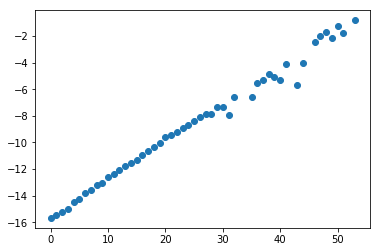
\includegraphics[scale=.5]{img/x-xge.png}
            \caption{ \( \log((x-x_{ge})_i) \) vs. \( i \) for \( i=1,2,...,m \)}
            \label{x-xge}
        \end{figure}

        However, QR factorization is backward stable, and so as expected we have a much lower error.


    \item[(c)] We start with the \( 5\times 5 \) matrix below.
    {\footnotesize
    \begin{align*}
        A = 
        \left[\begin{array}{rrrrr}
            1 &&&&1\\
            -1 & 1 &&&1 \\
            -1 & -1 & 1&&1 \\
            -1 & -1 & -1 & 1 & 1\\
            -1 & -1 & -1 & -1 & 1\\
        \end{array}\right]
    \end{align*}
        }

    We do not require pivoting at the first step. We perform a row operation giving,

    {\footnotesize
    \begin{align*}
        \left[\begin{array}{rrrrr}
            1 \\
            1 & 1 \\
            1 & & 1 \\
            1 & & & 1 \\
            1 & & & & 1 
        \end{array}\right]
         \left[\begin{array}{rrrrr}
            1 &&&&1\\
            -1 & 1 &&&1 \\
            -1 & -1 & 1&&1 \\
            -1 & -1 & -1 & 1 & 1\\
            -1 & -1 & -1 & -1 & 1\\
        \end{array}\right]
       =
        \left[\begin{array}{ccccc}
            1 & 0 & 0 & 0 & 1 \\
            0 & 1 & 0 & 0 & 2 \\
            0 & -1 & 1 & 0 & 2 \\
            0 & -1 & -1 & 1 & 2 \\
            0 & -1 & -1 & -1 & 2 \\
        \end{array}\right]
    \end{align*}
    }

    We now pivot to move a ``2'' to the pivot position and apply another row operation,
    {\footnotesize
    \begin{align*}
        \left[\begin{array}{rrrrr}
            1 \\
            & 1 \\
            & -1& 1 \\
            & -1& & 1 \\
            & -1& & & 1 
       \end{array}\right]
         \left[\begin{array}{ccccc}
            1 & 0 & 0 & 0 & 1 \\
            0 & 1 & 0 & 0 & 2 \\
            0 & -1 & 1 & 0 & 2 \\
            0 & -1 & -1 & 1 & 2 \\
            0 & -1 & -1 & -1 & 2 \\
        \end{array}\right]
        \left[\begin{array}{rrrrr}
            1 \\
            & & & & 1 \\
            & & 1 \\
            & & & 1 \\
            & 1 
       \end{array}\right]
        =
         \left[\begin{array}{ccccc}
            1 & 1 & 0 & 0 & 0 \\
            0 & 2 & 0 & 0 & 1 \\
            0 & 0 & 1 & 0 & -2 \\
            0 & 0 & -1 & 1 & -2 \\
            0 & 0 & -1 & -1 & -2 \\
        \end{array}\right] 
   \end{align*}
   }

    We pivot again to move a ``-2'' to the pivot position, and apply another row operation,
    {\footnotesize
    \begin{align*}
        \left[\begin{array}{rrrrr}
            1 \\
            & 1 \\
            & & 1 \\
            & & -1 & 1 \\
            & & -1 & & 1 
        \end{array}\right]
        \left[\begin{array}{ccccc}
            1 & 1 & 0 & 0 & 0 \\
            0 & 2 & 0 & 0 & 1 \\
            0 & 0 & 1 & 0 & -2 \\
            0 & 0 & -1 & 1 & -2 \\
            0 & 0 & -1 & -1 & -2 \\
        \end{array}\right]
        \left[\begin{array}{rrrrr}
            1 \\
            & 1 \\
            & & & & 1 \\
            & & & 1 \\
            & &  1 
       \end{array}\right]
        =
        \left[\begin{array}{ccccc}
            1 & 1 & 0 & 0 & 0 \\
            0 & 2 & 1 & 0 & 0 \\
            0 & 0 & -2 & 0 & 1 \\
            0 & 0 & 0 & 1 & -2 \\
            0 & 0 & 0 & -1 & -2 \\
        \end{array}\right]
    \end{align*}
    }



    We pivot again and apply another row operation,
    {\footnotesize
    \begin{align*}
        \left[\begin{array}{rrrrr}
            1 \\
            & 1 \\
            & & 1 \\
            & & & 1 \\
            & & & -1 & 1 
        \end{array}\right]
         \left[\begin{array}{ccccc}
            1 & 1 & 0 & 0 & 0 \\
            0 & 2 & 1 & 0 & 0 \\
            0 & 0 & -2 & 0 & 1 \\
            0 & 0 & 0 & 1 & -2 \\
            0 & 0 & 0 & -1 & -2 \\
        \end{array}\right]
       \left[\begin{array}{rrrrr}
            1 \\
            & 1 \\
            & & 1 \\
            & & & & 1 \\
            & & & 1 
       \end{array}\right]
        =
        \left[\begin{array}{ccccc}
            1 & 1 & 0 & 0 & 0 \\
            0 & 2 & 1 & 0 & 0 \\
            0 & 0 & -2 & 1 & 0 \\
            0 & 0 & 0 & -2 & 1 \\
            0 & 0 & 0 & 0 & -2 \\
        \end{array}\right]
    \end{align*}
    }

    Therefore,
    {\footnotesize
        \begin{align*}
        U = 
         \left[\begin{array}{ccccc}
            1 & 1 & 0 & 0 & 0 \\
            0 & 2 & 1 & 0 & 0 \\
            0 & 0 & -2 & 1 & 0 \\
            0 & 0 & 0 & -2 & 1 \\
            0 & 0 & 0 & 0 & -2 \\
        \end{array}\right]
    \end{align*}
    }

    {\footnotesize
        \begin{align*}
        Q = 
       \left[\begin{array}{rrrrr}
            1 \\
            & & & & 1 \\
            & & 1 \\
            & & & 1 \\
            & 1 
       \end{array}\right]
       \left[\begin{array}{rrrrr}
            1 \\
            & 1 \\
            & & & & 1 \\
            & & & 1 \\
            & & 1 
       \end{array}\right]
       \left[\begin{array}{rrrrr}
            1 \\
            & 1 \\
            & & 1 \\
            & & & & 1 \\
            & & & 1 
       \end{array}\right]
        =
       \left[\begin{array}{rrrrr}
            1 \\
            & & 1 \\
            & & & 1 \\
            & & & & 1 \\
            & 1 
       \end{array}\right]
     \end{align*}
     }

     {\tiny
     \begin{align*}
         L&=
         \left[\begin{array}{rrrrr}
            1 \\
            1 & 1 \\
            1 & & 1 \\
            1 & & & 1 \\
            1 & & & & 1 
         \end{array}\right]^{-1}
        \left[\begin{array}{rrrrr}
            1 \\
            & 1 \\
            & -1 & 1 \\
            & -1 & & 1 \\
            & -1 & & & 1 
        \end{array}\right]^{-1}
        \left[\begin{array}{rrrrr}
            1 \\
            & 1 \\
            & & 1 \\
            & & -1 & 1 \\
            & & -1 &  & 1 
        \end{array}\right]^{-1}
        \left[\begin{array}{rrrrr}
            1 \\
            & 1 \\
            & & 1 \\
            & & & 1 \\
            & & & -1 & 1 
        \end{array}\right]^{-1}
         \\&=
        \left[\begin{array}{rrrrr}
            1 \\
            -1 & 1 \\
            -1 & 1 & 1 \\
            -1 & 1 & 1 & 1 \\
            -1 & 1 & 1 & 1 & 1 
        \end{array}\right]
     \end{align*}
     }

     We finally verify that,
     \begin{align*}
        AQ = LU
     \end{align*}

     The growth factor is 2.

     Based on the repeated structure of the steps after the first, it is clear that any size matrix of this form will have a similar \( PAQ=LU \) decomposition. Therefore, for a larger matrix the growth factor would also be two. 

     Since the growth factor is constant, then we expect Gaussian elimination to be backward stable, and that our results be accurate.

\end{enumerate}

\end{solution}

\begin{problem}[Exercise 23.1]
Let \( A \) be a nonsingular square matrix and let \( A=QR \) and \( A^*A=U^*U \) be QR and Cholesky factorizations, respectively, with the usual normalizations \( r_{jj},u_{jj}>0 \). Is it true or false that \( R=U \).
\end{problem}

\begin{solution}[Solution]
We have, 
\begin{align*}
    A^*A = (QR)^*(QR) = R^*Q^*QR = R^*R
\end{align*}

Since \( R \) is upper triangular and \( r_{jj} > 0 \) this is a Cholesky decomposition. 

Obviously \( A^*A = (A^*A)^* \) and for \( u\neq 0 \), \( u^*(A^*A)u = (u^*A^*)(Au) = (Au)^*(Au) = \norm{Au}^2 > 0 \). Thus \( A^*A \) is Hermetian positive definite and therefore has a unique Cholesky decomposition. This proves \( R=U \). \qed
\end{solution}

\begin{problem}[Exercise 24.1]
For each of the following statements, prove it is true or give an example to show it is false. Throughout, \( A\in\CC^{m\times m} \) unless otherwise indicated, and ``ew'' stands for eigenvalue.
    \begin{enumerate}
        \item[(a)] If \( \lambda \) is an ew of \( A \) and \( \mu\in\CC \), then \( \lambda-\mu \) is an ew of \( A-\mu I \).
        \item[(b)] If \( A \) is real and \( \lambda \) is an ew of \( A \), then so is \( -\lambda \).
        \item[(c)] If \( A \) is real and \( \lambda \) is an ew of \( A \), then so is \( \overline{\lambda} \). 
        \item[(d)] If \( \lambda \) is an ew of \( A \) and \( A \) is nonsingular, then \( \lambda^{-1} \) is an ew of \( A^{-1} \).
        \item[(e)] If all the ew's of \( A \) are zero, then \( A=0 \).
        \item[(f)] If \( A \) is hermetian and \( \lambda \) is an ew of \( A \), then \( |\lambda| \) is a singular value of \( A \).
        \item[(g)] If \( A \) is diagonalizable and all its ew's are equal, then \( A \) is diagonal.
   \end{enumerate}
\end{problem}

\begin{solution}[Solution]
We use the following equivalent statements:
\begin{itemize}[nolistsep]
    \item \( \lambda \) is an eigenvalue of \( A \) 
    \item \( \det(A-\lambda I) = 0 \).
    \item \( \lambda \) is a root of \( p_A(z) = \det(A-zI) \)
\end{itemize}

These are mostly trivial proofs, so I do not restate the above equivalences in each problem to exactly match the wording of the problem statement.

\begin{enumerate}
    \item[(a)] True. 
        \( \operatorname{det}((A-\mu I)-(\lambda-\mu)I) = \operatorname{det}(A-\mu I - \lambda I -(-\mu I)) = \operatorname{det}( A-\lambda I ) = 0 \) %, so \( \lambda-\mu \) is an eigenvector of \( A-\mu I \).
    \item[(b)] False. Consider \( A=[1]\in\RR^{1\times 1} \). Clearly \( \det(A-1 I) = 0 \) but \( \det(A-(-1)I) = 2 \neq 0 \).
    \item[(c)] True. If \( A \) is real then \( p_A(z) \) has real coefficients. Therefore, by the fundamental theorem of algebra, if \( \lambda \) is a root of \( p_A \), then so is \( \overline{\lambda} \).
    \item[(d)] True. \( Av = \lambda v \Longleftrightarrow  \lambda^{-1}A^{-1}Av = \lambda^{-1}A^{-1} \lambda v \Longleftrightarrow \lambda^{-1}v = \lambda^{-1}\lambda A^{-1} v \Longleftrightarrow A^{-1} v = \lambda^{-1}v \) 
    \item[(e)] False. Consider \( A=[[0,1],[0,0]] \) with \( p_A(z) = z^2 \) so all eigenvalues are zero. However, clearly \( A\neq 0 \). 
    \item[(f)] True. A Hermetian matrix is unitary diagonalizable as \( A=Q\Lambda Q^* \). Let \( S \) be the diagonal matrix with \( S_{i,i} = \operatorname{sign}(\Lambda_{i,i}) \). Then \( A= (SQ) (S\Lambda) Q^* = (SQ)|\Lambda|Q^* \) is an SVD of \( A \). This proves the singular values of \( A \) are the absolute values of the eigenvalues of \( A \).
    \item[(g)] True. All eigenvalues of \( A \) equal means \( A=\lambda I \). If \( A \) is unitarily diagonalizable, then there is some \( D \), diagonal, and \( Q \), unitary, such that \( D=QAQ^*  = Q(\lambda I)Q^* = \lambda QQ^* = \lambda I = A \).  
\end{enumerate}

\end{solution}

\begin{problem}[Exercise 24.2]
Here is Gerschgorin's theorem, which holds for any \( m\times m \) matrix \( A \): Every eigenvalue of \( A \) lies in at least one of the \( m \) circular disks in the complex plane with centers \( a_{ii} \) and radii \( \sum_{j\neq i} |a_{ij}| \). Moreover, if \( n \) of these disks form a connected domain that is disjoint from the other \( m-n \) disks, then there are precisely \( n \) eigenvalues of \( A \) within this domain.
\begin{enumerate}
    \item[(c)] Give estimates based on Gerschgorian's theorem for the eigenvalues of
        \begin{align*}
            A=\left[\begin{array}{rrr}8&1&0\\1&4&\epsilon\\0&\epsilon&1\end{array}\right], \qquad |\epsilon|<1
        \end{align*}
    \item[(d)] Find a way to establish the tighter bound \( |\lambda_3-1|\leq \epsilon^2 \) on the smallest eigenvalue of \( A \).
\end{enumerate}
\end{problem}

\begin{solution}[Solution]
\begin{enumerate}
    \item[(c)] Let \( \mathcal{D}(c,r) = \{z : |z-c|\leq r\} \) be the closed disk of radius \( r \) centered at \( c \). Then there is exactly one eigenvalue in each of the following three disks as no two disks intersect.
        \begin{align*}
            \mathcal{D}(8,1) && \mathcal{D}(4,1+|\epsilon|) && \mathcal{D}(1,|\epsilon|)    
        \end{align*}

        Since \( A \) is symmetric (and therefore Hermetian), we know all eigenvalues are real. We therefore take the part of the real axis contained in the above disks. This corresponds to the closed intervals,
        \begin{align*}
            [7,9] && [3-|\epsilon|,5+|\epsilon|] && [1-|\epsilon|,1+|\epsilon|]
        \end{align*}
    
    \item[(d)]
        Define,
        \begin{align*}
            Q=
            \left[\begin{array}{rrr}
                \epsilon^{-1} & \\
                & \epsilon^{-1} \\
                & & 1
            \end{array}\right]
            && Q^{-1} =
            \left[\begin{array}{rrr}
                \epsilon\\
                & \epsilon\\
                & & 1
            \end{array}\right]
        \end{align*}

        Then,
        \begin{align*}
            QAQ^{-1} = 
            \left[\begin{array}{rrr}
                8 & 1  \\
                1 & 4 & 1 \\
                & \epsilon^2 & 1
            \end{array}\right]
        \end{align*}

        
        Since \( QAQ^{-1} \) is a similarity transform of \( A \), \( QAQ^{-1} \) and \( A \) share eigenvalues. In particular, this means the eigenvalues of \( QAQ^{-1} \) are real.  
                Now note that since \( |\epsilon|<1 \) the Gershgorin row disks are disjoint. Therefore, the smallest eigenvalue of \( QAQ^{-1} \) is in the interval \( [1-\epsilon^2,1+\epsilon^2] \).
        
        This proves that the smallest eigenvector of \( A \) satisfies \( |\lambda_3-1|\leq \epsilon^2 \).

\end{enumerate}
\end{solution}



\begin{problem}[Exercise 6]
By hand, find a Householder reflector \(Q\) and an upper Hessenberg matrix \(H\) such that \(Q^{*} A Q = H\), where
\[ A = \left[ \begin{array}{ccc} 1 & 2 & 3 \\ 1 & 1 & 2 \\ 1 & 1 & 1 \end{array} \right]  \]
\end{problem}

\begin{solution}[Solution]
ince \( A \) is \( 3\times 3 \) it takes only Householder reflector to take \( A \) to an upper Hessenberg matrix.

First let,
\begin{align*}
    x = A_{2:3,1} = \left[\begin{array}{r}1\\1\end{array}\right]
\end{align*}

Now let,
\begin{align*}
    v = \operatorname{sign}(x_1)\norm{x}_2 e_1+x = 1 \sqrt{2} e_1 + x = \left[\begin{array}{r} \sqrt{2}+1\\1\end{array}\right]
\end{align*}

Then,
\begin{align*}
    Q = \left[\begin{array}{rr}I_1 & 0 \\ 0 & I_2-2\dfrac{vv^*}{v^*v} \end{array}\right] 
        = \left[
\begin{array}{rrr}
 1 & 0 & 0 \\
 0 & 1-\frac{2 \left(\sqrt{2}+1\right)^2}{\left(\sqrt{2}+1\right)^2+1} & -\frac{2 \left(\sqrt{2}+1\right)}{\left(\sqrt{2}+1\right)^2+1} \\
 0 & -\frac{2 \left(\sqrt{2}+1\right)}{\left(\sqrt{2}+1\right)^2+1} & 1-\frac{2}{\left(\sqrt{2}+1\right)^2+1} \\
\end{array}
    \right]
\end{align*}

Finally,
\begin{align*}
    H=Q^*AQ = 
    \left[
        \begin{array}{rrr}
 1 & -5/\sqrt{2} & 1/\sqrt{2} \\
 -\sqrt{2} & 5/2 & -1/2 \\
 0 & 1/2 & -1/2 \\
\end{array}
    \right]
\end{align*}
\end{solution}





\end{document}
